%
% Optional reading
%

\begin{frame}[plain,c]
\begin{center}
{\Huge \bf Optional reading for Lecture \thislecture}
\end{center}
\end{frame}


%
%
%

\begin{frame}{The electrostatic potential energy is stored in the field}

We can now prove a statement I made earlier: That {\bf the electrostatic potential energy is stored in the electric field}.\\
\vspace{0.1cm}
The potential energy stored in a system of N charges can be written as:
\begin{equation*}
   U = \frac{1}{2} \sum_{i,j=1;i{\ne}j}^{N} \frac{q_i q_j}{4\pi\epsilon_0|\vec{r}_{ij}|}
     = \frac{1}{2} \sum_{i}^{N} q_i {\color{red}\sum_{j=1;j{\ne}i}^{N} \frac{q_j}{4\pi\epsilon_0|\vec{r}_{ij}|}}
     = \frac{1}{2} \sum_{i}^{N} q_i {\color{red}V(\vec{r}_{i})}
\end{equation*}

where
\begin{equation*}
   V(\vec{r}_{i}) = \sum_{j=1;j{\ne}i}^{N} \frac{q_j}{4\pi\epsilon_0|\vec{r}_{ij}|}
\end{equation*}
is the potential at $\vec{r}_{i}$ due to all charges other than $q_i$.\\

\vspace{0.2cm}

The above result can be adapted for the continuous case too, using the (by now) familiar substitutions:
\begin{equation*}
   U = \frac{1}{2} \sum_{i}^{N} q_i V(\vec{r}_{i}) \rightarrow \frac{1}{2} \int_{V} \rho(\vec{r}) V(\vec{r}) d\tau
\end{equation*}

\end{frame}

%
%
%

\begin{frame}{The electrostatic potential energy is stored in the field}

The expression we have for the potential energy U of a continuous charge
distribution described by charge density $\rho$ is:
\begin{equation*}
   U = \frac{1}{2} \int_{V} \rho(\vec{r}) V(\vec{r}) d\tau
\end{equation*}
We will show that U is related to a volume integral of $|\vec{E}|^2$.\\

\vspace{0.3cm}

Using Gauss's law, the charge density $\rho$ can be written as:
\begin{equation*}
   \vec{\nabla} \vec{E}(\vec{r}) = \frac{\rho(\vec{r})}{\epsilon_0} \Rightarrow \rho(\vec{r}) = \epsilon_0 \vec{\nabla} \vec{E}(\vec{r})
\end{equation*}

Substituting $\rho$ into the expression for U, we have:
\begin{equation*}
   U = \frac{\epsilon_0}{2} \int_{V} \Big(\vec{\nabla} \vec{E}(\vec{r})\Big) V(\vec{r}) d\tau
\end{equation*}

\end{frame}

%
%
%

\begin{frame}{The electrostatic potential energy is stored in the field}

I would like to express U in terms of $\vec{E}$ only.\\
\vspace{0.2cm}
Since $\vec{\nabla} V = - \vec{E}$, I will try to move the $\vec{\nabla}$ in the previous
expression so that it operates on V instead on $\vec{E}$.\\
\vspace{0.2cm}
The trick is to operate with $\vec{\nabla}$ on the product $\vec{E} V$:
\begin{equation*}
  \vec{\nabla} \Big(\vec{E}(\vec{r}) V(\vec{r}) \Big) =
     \Big(\vec{\nabla} \vec{E}(\vec{r}) \Big) V(\vec{r}) + \vec{E}(\vec{r}) \Big(\vec{\nabla} V(\vec{r}) \Big) \Rightarrow
\end{equation*}
\begin{equation*}
   \Big(\vec{\nabla} \vec{E}(\vec{r}) \Big) V(\vec{r}) =
      \vec{\nabla} \Big(\vec{E}(\vec{r})) V(\vec{r}) \Big) - \vec{E}(\vec{r}) \Big(\vec{\nabla} V(\vec{r}) \Big)
\end{equation*}

Substituting the above in the last equation of the previous page we have:
\begin{equation*}
   U = \frac{\epsilon_0}{2} \int_{V} \vec{\nabla} \Big(\vec{E}(\vec{r})) V(\vec{r}) \Big) d\tau -
       \frac{\epsilon_0}{2} \int_{V} \vec{E}(\vec{r}) \Big(\vec{\nabla} V(\vec{r}) \Big)  d\tau
\end{equation*}

\end{frame}


%
%
%

\begin{frame}{The electrostatic potential energy is stored in the field}

Using Gauss' theorem, the 1$^{st}$ term of the previous expression for U becomes:
\begin{equation*}
   \int_{V} \vec{\nabla} \Big(\vec{E}(\vec{r})) V(\vec{r}) \Big) d\tau =
   \oint_{S} \Big(\vec{E}(\vec{r})) V(\vec{r}) \Big) d\vec{S}
\end{equation*}

Using $\vec{\nabla} V = - \vec{E}$, the 2$^{nd}$ term of the previous expression for U becomes:
\begin{equation*}
   \int_{V} \vec{E}(\vec{r}) \Big(\vec{\nabla} V(\vec{r}) \Big) d\tau =
  -\int_{V} \vec{E}(\vec{r}) \vec{E}(\vec{r}) d\tau =
  -\int_{V} |\vec{E}(\vec{r})|^{2} d\tau
\end{equation*}

The equation for the electric potential U can be rewritten as:
\begin{equation*}
   U = \frac{\epsilon_0}{2} \oint_{S} \Big(\vec{E}(\vec{r})) V(\vec{r}) \Big) d\vec{S} +
       \frac{\epsilon_0}{2} \int_{V} |\vec{E}(\vec{r})|^2  d\tau
\end{equation*}

As r $\rightarrow\infty$, the surface term $\oint_{S} \Big(...\Big) d\vec{S}$ $\rightarrow$ 0.
Therefore:
\begin{equation*}
   U = \frac{\epsilon_0}{2} \int_{all\;space} |\vec{E}(\vec{r})|^2  d\tau
\end{equation*}

\end{frame}


%
%
%

\begin{frame}{The Dirichlet boundary condition yields unique solutions}

This can be understood as follows:\\
\begin{itemize}
{\small
  \item Imagine a volume with a charge density $\rho$ which is known at all points.
  \item Also assume that the potential is known everywhere on the boundaries (i.e. on the surface surrounding the volume)
  \item Assume that there are two distinct solutions, $V_{1}(\vec{r})$ and $V_{2}(\vec{r})$.
    \begin{itemize}
    {\small
       \item $\vec{\nabla}^{2}V_1(\vec{r}) = -\rho(\vec{r})/\epsilon_0$
       \item $\vec{\nabla}^{2}V_2(\vec{r}) = -\rho(\vec{r})/\epsilon_0$
    }
    \end{itemize}
  \item Now, consider the function $V_{3}(\vec{r}) = V_{1}(\vec{r}) - V_{2}(\vec{r})$
    \begin{itemize}
    {\small
      \item At the boundary, $V_{3}(\vec{r}) = 0$ (since both $V_1$, $V_2$ satisfy the same boundary condition)
      \item Also, $V_{3}(\vec{r})$ satisfies the equation $\vec{\nabla}^{2}V_{3} = 0$ and, as such, changes monotonically inside the volume and has no minima/maxima.
    }
    \end{itemize}
  \item $V_3$ ranges between 0 and ...0, so $V_3$ is 0 everywhere in the given volume.
  \item This contradicts the assumption that two distinct solutions $V_1$, $V_2$ can exist.
        $V_1 = V_2$ everywhere in the volume, so a unique solution exists.
    \begin{equation*}
      \vec{\nabla}^{2}V_{3} = \vec{\nabla}^{2}(V_1-V_2) = \vec{\nabla}^{2}V_1 - \vec{\nabla}^{2}V_2 = - \frac{\rho}{\epsilon_0} + \frac{\rho}{\epsilon_0} = 0
    \end{equation*}
}
\end{itemize}

\end{frame}

% ------------------------------------------------------------------------------

%
% Worked example :
%

{
\problemslide

%
%
%

\begin{frame}{Worked example: Hypothetical form of electric force}

  \begin{blockexmplque}{Question}
    Suppose that instead of the Coulomb force law, one found experimentally
    that the force between two charges $q_1$ and $q_2$ was
    \begin{equation*}
        \vec{F}_{12} = \frac{q_1 q_2}{4\pi \epsilon_0}
         \frac{1 - \sqrt{C|\vec{r}_1-\vec{r}_2|}}{|\vec{r}_1-\vec{r}_2|^3}
          (\vec{r}_1-\vec{r}_2)
    \end{equation*}
    where $C$ is a constant.
    \begin{itemize}
      \item
      Find an expression for the electric field $\vec{E}$
      surrounding a point charge $q$ at the origin of the coordinate system.
      \item
      Choose an arbitrary closed path around a point charge $q$ and calculate
      the line integral $\oint \vec{E} \cdot d\vec{\ell}$.
      Compare with the Coulomb result.
      \item
      Find $\oint \vec{E} \cdot d\vec{S}$ over a spherical surface of radius
      $R$ with a point charge $q$ at its centre.
      Compare with the Coulomb result.
      \item
      Calculate $\vec{\nabla} \cdot \vec{E}$ and compare with the Coulomb result.
    \end{itemize}
  \end{blockexmplque}

\end{frame}

%
%
%

\begin{frame}{Worked example: Hypothetical form of electric force}

  Assuming, without loss of generality, that the
  point charge $q$ is at the origin of the coordinate system
  and that a positive test charge $Q$
  is brought at distance $\vec{r}$ from $q$,
  the electric field at $\vec{r}$ is given by:
  \begin{equation*}
    \vec{E}(\vec{r}) = \frac{\vec{F}_{Qq}}{Q}
  \end{equation*}
  where $\vec{F}_{Qq}$ is the force exerted on $Q$ because of $q$.

  Using the given expression of the electric force,
  and using $r=|\vec{r}|$,
  $\vec{F}_{Qq}$ can be written as:
  \begin{equation*}
    \displaystyle
    \vec{F}_{Qq} =
      \frac{Qq}{4\pi \epsilon_0}
      \frac{1-\sqrt{Cr}}{r^3} \vec{r}
      \xRightarrow{\;\; \vec{r} = r \hat{r} \;\;}
      \vec{F}_{Qq} =
        \frac{Qq}{4\pi \epsilon_0}
        \frac{1-\sqrt{Cr}}{r^2} \hat{r}
  \end{equation*}

  Therefore, the electric field at point $\vec{r}$ can be written as:
  \begin{equation*}
    \displaystyle
    \vec{E}(\vec{r}) =
        \frac{q}{4\pi \epsilon_0}
        \frac{1-\sqrt{Cr}}{r^2} \hat{r}
  \end{equation*}

\end{frame}

%
%
%

\begin{frame}{Worked example: Hypothetical form of electric force}

  The path integral of the electric field along a closed path L
  can be written as:
  \begin{equation*}
    \oint_{L} \vec{E} \cdot d\vec{\ell} =
       \frac{q}{4\pi \epsilon_0}
         \oint_{L} \frac{1-\sqrt{Cr}}{r^2} \hat{r} \cdot d\vec{\ell}
  \end{equation*}

  Using:
  \begin{equation*}
    \hat{r} \cdot d\vec{\ell} = d\ell cos\theta = dr
  \end{equation*}

  we find:
  \begin{equation*}
    \oint_{L} \vec{E} \cdot d\vec{\ell} =
       \frac{q}{4\pi \epsilon_0}
         \oint_{L} \frac{1-\sqrt{Cr}}{r^2} dr =
        \frac{q}{4\pi \epsilon_0}
           \oint_{L} \Big(r^{-2} - \sqrt{C} r^{-3/2}\Big) dr
  \end{equation*}

  \begin{equation*}
      = \frac{q}{4\pi \epsilon_0}
          \Big(-\frac{1}{r^\prime}+2\sqrt{C}\frac{1}{\sqrt{r^\prime}}\Big)
            \Bigg\rvert_{r}^{r} = 0
  \end{equation*}

  This is the same as the corresponding Coulomb result.

\end{frame}

%
%
%

\begin{frame}{Worked example: Hypothetical form of electric force}

  The flux of the electric field through the
  closed surface $S$ or a sphere with radius $R$ can be written as:
  \begin{equation*}
    \oint_{S(R)} \vec{E} \cdot d\vec{S} =
       \frac{q}{4\pi \epsilon_0}
         \oint_{S(R)} \frac{1-\sqrt{Cr}}{r^2} \hat{r} \cdot d\vec{S}
  \end{equation*}

  Since the integration surface is a sphere centred at the origin
  of the coordinate system, $d\vec{S}$ is a radial vector:
  \begin{equation*}
    d\vec{S} = dS \hat{r}
  \end{equation*}

  and, therefore, the surface integral can be written as:
  \begin{equation*}
    \oint_{S(R)} \vec{E} \cdot d\vec{S} =
       \frac{q}{4\pi \epsilon_0}
         \oint_{S(R)} \frac{1-\sqrt{Cr}}{r^2} dS
  \end{equation*}

  Over the integration surface, at $r=R$ the integrand has a
  constant value of:
  $\displaystyle \frac{q}{4\pi \epsilon_0} \frac{1-\sqrt{CR}}{R^2}$.

\end{frame}

%
%
%

\begin{frame}{Worked example: Hypothetical form of electric force}

  Therefore, the expression for electric flux through $S$ becomes:
  \begin{equation*}
    \oint_{S(R)} \vec{E} \cdot d\vec{S} =
       \frac{q}{4\pi \epsilon_0}
         \frac{1-\sqrt{CR}}{R^2}
           \oint_{S(R)} dS =
        \frac{q}{4\pi \epsilon_0}
          \frac{1-\sqrt{CR}}{\cancel{R^2}} 4\pi\cancel{R^2} \Rightarrow
  \end{equation*}
  \begin{equation*}
    \oint_{S(R)} \vec{E} \cdot d\vec{S} =
        \frac{q}{\epsilon_0} \Big(1-\sqrt{CR}\Big)
  \end{equation*}

  This differs by corresponding Coulomb result:
  Therefore, the expression for electric flux through $S$ becomes:
  \begin{equation*}
    \oint_{S(R)} \vec{E} \cdot d\vec{S} = \frac{q}{\epsilon_0}
  \end{equation*}

  by a term equal to
  $\displaystyle -\sqrt{CR} \frac{q}{\epsilon_0}$.

\end{frame}

%
%
%

\begin{frame}{Worked example: Hypothetical form of electric force}

  The given electric field is a radial one and,
  therefore, it is easier to compute its divergence by expressing
  the divergence operator in spherical coordinates:
  \begin{equation*}
    \vec{\nabla} \cdot \vec{E} =
     \frac{1}{r^2} \frac{\partial}{\partial r}
      \Bigg( r^2
        \Big(
          \frac{q}{4\pi \epsilon_0}
          \frac{1-\sqrt{Cr}}{r^2}
        \Big)
      \Bigg)
  \end{equation*}

  Therefore:
  \begin{equation*}
    \vec{\nabla} \cdot \vec{E} =
      \frac{q}{4\pi \epsilon_0}
      \frac{1}{r^2}
      \frac{\partial}{\partial r}
      \Big( 1-\sqrt{Cr} \Big) =
      \frac{q}{4\pi \epsilon_0}
      \frac{1}{r^2}
      \Big(-\frac{1}{2}\sqrt{\frac{C}{r}} \Big) =
      - \frac{q \sqrt{C}}{8\pi \epsilon_0 r^{5/2}}
  \end{equation*}

  This differs from the Coulomb result:
  \begin{equation*}
    \vec{\nabla} \cdot \vec{E} = \frac{\rho}{\epsilon_0}
  \end{equation*}
  which, for a point charge q at the origin, can be written as
  \begin{equation*}
    \vec{\nabla} \cdot \vec{E} = \frac{q}{\epsilon_0} \delta(r)
  \end{equation*}

\end{frame}

} %\problemslide

% ------------------------------------------------------------------------------
% ------------------------------------------------------------------------------

%
% Worked example :
%

{
\problemslide

\begin{frame}{Worked example: Potential $V$ and field $\vec{E}$ of charged disc}

  \begin{blockexmplque}{Question}
    \begin{columns}
      \begin{column}{0.60\textwidth}
        The figure on the right shows a plastic disc of radius $R$,
        charged on its top surface to a uniform surface charge density $\sigma$.
        \begin{itemize}
        \item
        Find the electrostatic potential $V$ at point $P$ on the
        central axis of the disc.
        \item
        Using the expression for $V$, calculate
        the electric field $\vec{E}$ at point $P$.
        \end{itemize}
      \end{column}
      \begin{column}{0.40\textwidth}
        \begin{center}
          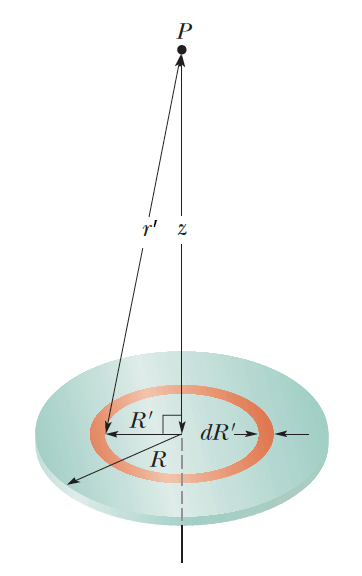
\includegraphics[width=0.92\textwidth]{./images/problems/lect03_charged_disk_3}\\
        \end{center}
      \end{column}
    \end{columns}
  \end{blockexmplque}

\end{frame}

%
%
%

\begin{frame}{Worked example: Potential $V$ and field $\vec{E}$ of charged disc}

  The electric field $V$ at the point $\vec{r}$, due to a continuous
  distribution of charge is given by:
  \begin{equation*}
    V(\vec{r}) = \frac{1}{4\pi\epsilon_0}
     \int \frac{dq(\pvec{r}')}{|\vec{r}-\pvec{r}'|}
  \end{equation*}

  Taking the point $P$ to be at the origin of the coordinate system,
  we have $\vec{r}=\vec{0}$ and, therefore, the above expression simplifies to:
  \begin{equation*}
    V = \frac{1}{4\pi\epsilon_0}
     \int \frac{dq(\pvec{r}')}{|\pvec{r}'|}
  \end{equation*}

  Integrating $dq(\pvec{r}')$ over a ring with radius $R'$ and width $dR'$,
  concentric with the plastic disk, we obtain:
  \begin{equation*}
    dq(R') = \int_{R'}^{R'+dR'} dq(\pvec{r}') = \sigma 2\pi R' dR'
  \end{equation*}
  where:
  \begin{equation*}
    |\pvec{r}'| = \sqrt{R'^2+z^2}
  \end{equation*}

\end{frame}

%
%
%

\begin{frame}{Worked example: Potential $V$ and field $\vec{E}$ of charged disc}

  Therefore, the potential $V$ can be written as:
  \begin{equation*}
    V =
     \frac{1}{4\pi\epsilon_0}
       \int_{0}^{R} \frac{\sigma 2\pi R' dR'}{\sqrt{R'^2+z^2}} =
     \frac{\sigma}{2\epsilon_0}
       \int_{0}^{R} \frac{R' dR'}{\sqrt{R'^2+z^2}}
  \end{equation*}

  Carrying out the integration, we find:
  \begin{equation*}
    V =
     \frac{\sigma}{2\epsilon_0}
       \frac{1}{2} \int_{0}^{R} \frac{d(R'^2+z^2)}{\sqrt{R'^2+z^2}}
  \end{equation*}

  \begin{equation*}
    V =
     \frac{\sigma}{2\epsilon_0}
       \frac{1}{2} 2 \sqrt{R'^2+z^2}\Big\rvert_{0}^{R} \Rightarrow
  \end{equation*}

  \begin{equation*}
    V =
     \frac{\sigma}{2\epsilon_0}
       \Big( \sqrt{R^2+z^2} - z \Big)
  \end{equation*}

\end{frame}

%
%
%

\begin{frame}{Worked example: Potential $V$ and field $\vec{E}$ of charged disc}

  The electric field $\vec{E}$ is computed from the electric potential $V$ as:
  \begin{equation*}
    \vec{E} = -\vec{\nabla} V
  \end{equation*}

  The $x$ and $y$ components of $\vec{E}$ vanish at $P$
  by symmetry and, therefore:
  \begin{equation*}
    \vec{E} = - \frac{\partial V}{\partial z} \hat{z}
  \end{equation*}

  \begin{equation*}
    \frac{\partial V}{\partial z} =
    \frac{\partial}{\partial z}
    \Big\{ \frac{\sigma}{2\epsilon_0} \Big( \sqrt{R^2+z^2} - z \Big) \Big\} =
    \frac{\sigma}{2\epsilon_0} \Big\{ \frac{z}{\sqrt{R^2+z^2}} - 1 \Big\}
  \end{equation*}

  \begin{equation*}
    \vec{E} = \frac{\sigma}{2\epsilon_0}
       \Big\{ 1 - \frac{z}{\sqrt{R^2+z^2}} \Big\} \hat{z}
  \end{equation*}

\end{frame}

} %\problemslide

% ------------------------------------------------------------------------------
% ------------------------------------------------------------------------------

%
%
%

{
\programmingslide

%
%
%

\begin{frame}{PHYS201 scientific programming task for Lecture \thislecture}

{\small

We will attempt to {\bf solve numerically the Laplace equation in 2-D},
for some given boundary conditions, and determine the potential V!\\
\vspace{0.2cm}
The Laplace equation in 2-D takes the form
\begin{equation*}
  \frac{\partial^2 V(x,y)}{\partial x^2} +
  \frac{\partial^2 V(x,y)}{\partial y^2} = 0
\end{equation*}
\vspace{0.2cm}
We will solve this equation for all x, y in the square area defined by:
\begin{equation*}
    0 < x < L \;\;\; \text{and} \;\;\; 0 < y < L
\end{equation*}
\vspace{0.2cm}
Our boundary conditions are:
\begin{equation*}
    V(x,0) = V_0, \;\;\; V(x,L) = 0,  \;\;\; V(0,y) = 0,  \;\;\; V(L,y) = 0
\end{equation*}
Take L = 1 m and V$_0$ = 1 V.
}
\end{frame}

%
%
%

\begin{frame}{PHYS201 scientific programming task for Lecture \thislecture}

{\small

{\bf \color{red}Hint:} Solve the Laplace equation numerically,
using the {\em finite difference method}.

Consider the Taylor expansions of a function f(x) around x:
\begin{equation*}
   f(x+h) = f(x) + h f^{\prime}(x) + \frac{h^2}{2} f^{\prime \prime}(x) + O(h^3)
\end{equation*}
\begin{equation*}
   f(x-h) = f(x) - h f^{\prime}(x) + \frac{h^2}{2} f^{\prime \prime}(x) - O(h^3)
\end{equation*}
where h is a small distance.\\
\vspace{0.2cm}
Adding the two equations, we obtain the
{\em first central difference approximation} for the second derivative of f(x):
\begin{equation*}
   f(x+h) + f(x-h) = 2f(x) + h^2 f^{\prime \prime}(x) + O(h^4) \Rightarrow
\end{equation*}
\begin{equation*}
   f^{\prime \prime}(x) = \frac{f(x+h) - 2f(x) + f(x-h)}{h^2} + O(h^2)
\end{equation*}
}
\end{frame}

%
%
%

\begin{frame}{PHYS201 scientific programming task for Lecture \thislecture}

{\small

\begin{columns}
  \begin{column}{0.25\textwidth}
   \begin{center}
     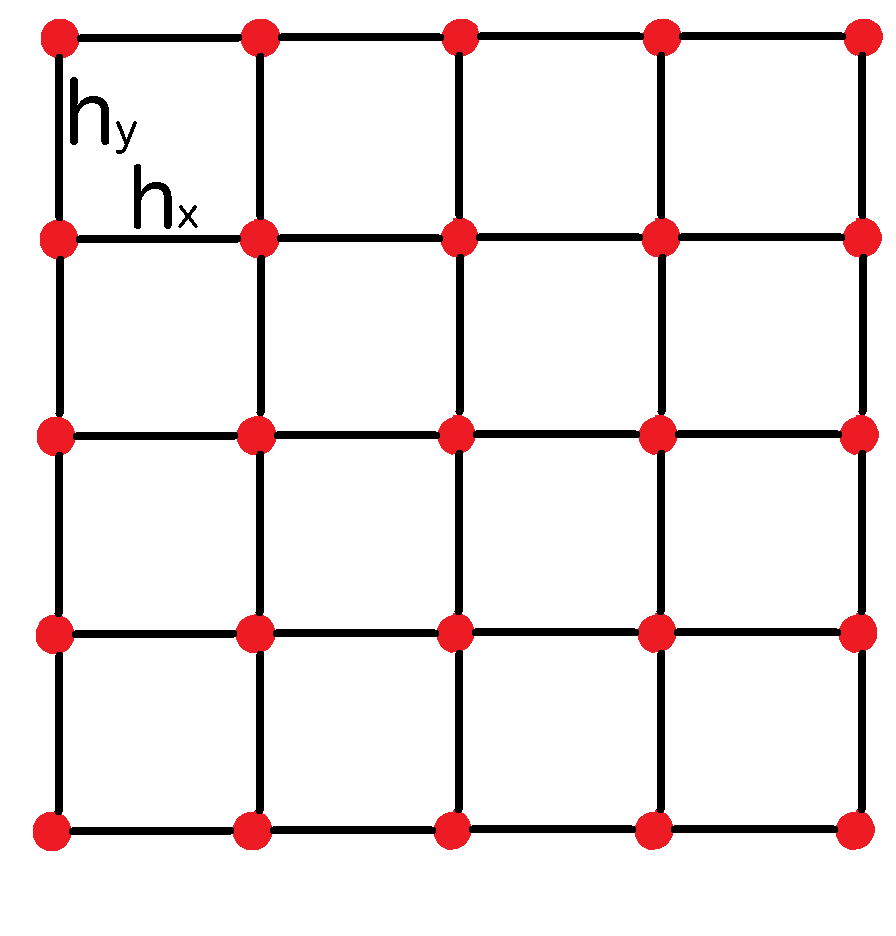
\includegraphics[width=0.90\textwidth]{./images/problems/lect03_computing_grid2d.png}
   \end{center}
  \end{column}
  \begin{column}{0.75\textwidth}
    Now, consider a uniform mesh (grid), as shown on the left,
    where the spacing between neighbouring points along x is h$_x$
    and the spacing between neighbouring points along y is h$_y$.\\
    \vspace{0.2cm}
    Using the {\em first central difference approximation},
    the Laplace equation for any point on the 2-D grid can be written as:
  \end{column}
\end{columns}

\begin{equation*}
   \frac{V(x+h_x,y) - 2V(x,y) + V(x-h_x, y)}{h_x^2} +
   \frac{V(x,y+h_y) - 2V(x,y) + V(x, y-h_y)}{h_y^2} = 0
\end{equation*}

If the grid is uniform (h$_x$ = h$_y$ = h), then the above equation becomes:
\begin{equation*}
   V(x+h,y) + V(x-h, y) +
   V(x,y+h) + V(x, y-h) - 4V(x,y) = 0
\end{equation*}

You have a set of such equations, one for each grid point, which you need
to {\bf solve simultaneously} in order to determine V(x,y) for each grid point.
}
\end{frame}


} % programming

% ------------------------------------------------------------------------------
% ------------------------------------------------------------------------------
